\section{From mixed amplification to an independent-site kernel}
\label{sec:graph}

The mixed amplification has eliminated the unit-modulus label $g_x$ by
Cauchy--Schwarz. Its positive square $I_{2,x}$ contains only the centered
label $F_x$. We first turn its off-diagonal terms into edges between
integers at small additive distance. We then separate the residue data at
the endpoints from the additional residue data in each representation of
an edge. Throughout this section, all parameters other
than $B$ and $x$ are fixed; $x$ tends to infinity first. Constants are
uniform when the smooth scale variable belongs to the compact range
specified below.

\subsection{The change of variables}

Consider distinct coefficients $a,b$ in the inner square defining
$I_{2,x}$, for fixed $m,c$, and put $l_a=(am+1)/c$ and
$l_b=(bm+1)/c$. The congruences imply that $m$ is a unit modulo $c$
and that
\[
 a-b=jc,\qquad 0<|j|\le T.
\]
They also imply $(a,c)=(b,c)=1$. Since $a,b$ are rough and
$|j|\le T<P_0$, we have $(a,j)=(b,j)=1$, and hence $(a,b)=1$.
For the ordered term in which the $a$-factor is conjugated, set
\[
 n'=b l_a,\qquad n'+j=a l_b.
\]
For these fixed coefficients, this is a bijective reindexing by the
conditions $b\mid n'$ and $a\mid n'+j$. Indeed, write $n'=bz$.
The latter congruence, together with $b=a-jc$, gives
$j(1-cz)\equiv0\pmod a$. Thus
\[
 m=\frac{cz-1}{a}
\]
is an integer, and substitution recovers both original congruences and
both displayed identities. Positive compact scale supports ensure all
arguments are positive for large $x$.

Figure~\ref{fig:graph-reindexing} records the two fixed multiplications
that produce the additive shift. Only fixed-multiplier invariance is used;
the centered function $F_x$ need not be multiplicative.

\begin{figure}[htbp]
\centering
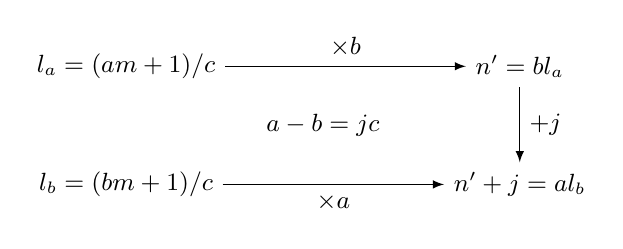
\begin{tikzpicture}[>=latex, every node/.style={font=\small}]
\node (la) at (0,0) {$l_a=(am+1)/c$};
\node (lb) at (0,-1.5) {$l_b=(bm+1)/c$};
\node (np) at (5,0) {$n'=bl_a$};
\node (nj) at (5,-1.5) {$n'+j=al_b$};
\draw[->] (la) -- node[above] {$\times b$} (np);
\draw[->] (lb) -- node[below] {$\times a$} (nj);
\draw[->] (np) -- node[right] {$+j$} (nj);
\node at (2.5,-0.75) {$a-b=jc$};
\end{tikzpicture}
\caption{The exact reindexing of two divisor representations. The
coefficient identity makes the new endpoints differ by $j$, while
fixed-multiplier invariance preserves their centered labels.}
\label{fig:graph-reindexing}
\end{figure}

For fixed $B$, the coefficient supports are finite, so
\eqref{eq:labels-multiplier} applies simultaneously to the multipliers
$c,b,a$ once $x$ is sufficiently large. Removing $c$ and then inserting
$b,a$ gives
\[
 \overline{F_x(am+1)}F_x(bm+1)
 =\overline{F_x(l_a)}F_x(l_b)
 =\overline{F_x(n')}F_x(n'+j).
\]
Define
\[
 \Psi_s(u_1,u_2)=
 \psi(u_1)\psi(u_2)\phi(s/u_1)\phi(s/u_2).
\]
If $s=n'/(Tx)$, $u_1=a/(Tc)$ and $u_2=b/(Tc)$, then
\[
 s/u_1=bm/x+b/(ax),\qquad s/u_2=am/x+1/x.
\]
The two original $\phi$-arguments are therefore interchanged, with
errors $O_B(1/x)$. Since they occur as a product, their replacement by
$\Psi_s$ has vanishing error for fixed $B$. There is a fixed compact
interval $\mathcal S\subset(0,\infty)$ outside which $\Psi_s$ vanishes
on the coefficient supports. It depends only on $\phi,\psi$.

Consequently, the off-diagonal part of $I_{2,x}/(BT)$ is, up to $o_x(1)$,
\begin{equation}\label{eq:16}
 \frac1{Tx}\sum_{n'}\sum_{0<|j|\le T}
 \overline{F_x(n')}F_x(n'+j)
       \mathcal K_j(n',n'/(Tx)),
\end{equation}
where, for $u\in\whZ$,
\begin{equation}\label{eq:17}
\begin{split}
 \mathcal K_j(u,s)=\frac1B
 \sum_{\substack{a-b=jc,\ (a,b)=(a,c)=(b,c)=1\\
                  b\mid u,\ a\mid u+j}}
 &A(a)A(b)A(c)K(u/b)K((u+j)/a)\\[-2pt]
 &\quad\cdot K\!\left(\frac{c(u/b)-1}{a}\right)
 \rho_0(\log c/B)\Psi_s(a/(Tc),b/(Tc)).
\end{split}
\end{equation}
All coefficient variables are positive integers. Divisibility in
$\whZ$ means membership in the image of multiplication by the
divisor; that multiplication is injective. The preceding congruence
calculation also proves that every quotient in \eqref{eq:17} is
defined on its summation domain. This kernel is nonnegative, depends
on finitely many prime-power residues, and satisfies
\[
 \mathcal K_j(u,s)=\mathcal K_{-j}(u+j,s).
\]
For this last identity, exchange $a,b$: the last quotient is unchanged
because $c(u+j)-a=cu-b$.

\begin{lemma}[Mean edge mass]\label{lem:graph-edge-mass}
Uniformly for $0<|j|\le T$ and $s\in\mathcal S$,
\begin{equation}\label{eq:18}
 \E_{u\in\whZ}\mathcal K_j(u,s)\ll\frac{\Sigma(j)}T.
\end{equation}
The implied constant can be independent of the regularity parameter
$C_*$.
\end{lemma}

\begin{proof}
Replace all truncated weights by their untruncated majorants.
For fixed pairwise coprime $a,b,c$, the two endpoint congruences have
Haar probability $1/(ab)$. At a prime $p\in\mathcal P$ not dividing
$abc$, the three residue weights have distinct zero classes
$0,-j,b/c$ for $u$. Here $p>|j|$, and $b/c\not\equiv-j\pmod p$
follows from $a=b+jc$. Their local mean is $1-3/(2p)$.
At primes dividing $abc$ discard the local reducing factors; this
changes the Euler-product bound by at most
$\exp(O(\sum_{p\mid abc}1/p))=O(1)$, since that sum is $O(B/P_0)$.
Independence over primes and Mertens' formula give
\[
 R^{3/2}\prod_{p\in\mathcal P}(1-3/(2p))\ll1.
\]
On a dyadic box $c\asymp X$, the denominator is
$ab\asymp T^2X^2$. The three-form estimate \eqref{eq:7} bounds its
contribution before the factor $1/B$ by $O(\Sigma(j)/T)$.
There are $O(B)$ boxes. This proves the assertion using only
untruncated upper bounds.
\end{proof}

\subsection{Blocks and the norm used for comparison}

Fix $0<\eta<1$ and $C_6>1$, and set $M=\lceil C_6T\rceil$.
Removing the lags $|j|<\eta T$ in \eqref{eq:16} costs
$O(\eta)+o_x(1)$ in absolute upper limit, by
Lemma~\ref{lem:graph-edge-mass} and the bounded ordinary averages of
$\Sigma$. Average the origins over $i=1,\ldots,M$, writing
$n'=n+i$. For fixed $B$, replacing $(n+i)/(Tx)$ by $n/(Tx)$
has vanishing error. At lag $j$, the fraction of $i$ for which
$k=i+j\notin[1,M]$ is at most $|j|/M$. The total cost of these
endpoints is $O(T/M)=O(1/C_6)$. The remaining expression is
\begin{equation}\label{eq:19}
 \mathcal Q^{\mathrm{arith}}_{B,x}:=\frac1{Tx}\sum_n\frac1M
 \sum_{\substack{1\le i,k\le M\\\eta T\le|k-i|\le T}}
 \overline{F_x(n+i)}F_x(n+k)
 \mathcal K_{k-i}(n+i,n/(Tx)).
\end{equation}
Thus \eqref{eq:15} and the diagonal estimate give a positive lower
bound for the iterated lower limit of \eqref{eq:19}, once $\eta$ is
small enough and $C_6$ is large enough. These choices are made after
$C_*$ and before letting $B$ grow.

Call a pair $(i,k)$ \emph{allowed} if
$1\le i,k\le M$ and $\eta T\le|k-i|\le T$. All matrices below are
zero on other pairs. For a real matrix $H$, define
\begin{equation}\label{eq:graph-cutnorm}
 \|H\|_\square=
 \frac1M\max_{\epsilon,\delta\in\{-1,1\}^M}
 \left|\sum_{i,k}H_{ik}\epsilon_i\delta_k\right|.
\end{equation}
The same maximum results from allowing real test coordinates in
$[-1,1]$. Splitting real and imaginary parts shows that for complex
$z_i$ with $|z_i|\le2$,
\begin{equation}\label{eq:graph-cut-labels}
 \left|\frac1M\sum_{i,k}H_{ik}\overline{z_i}z_k\right|
 \le16\|H\|_\square.
\end{equation}
For fixed $B$, a matrix whose entries are finite-residue functions
continuous in $s$ has the same property after taking this finite
maximum. Its ordinary scale averages converge to its Haar-product
integral. Therefore bounds on the Haar expectation of the norm,
uniformly for $s\in\mathcal S$, control errors in
\eqref{eq:19}. This comparison is deterministic in the labels; it
requires no independence between the labels and the residue data.

\subsection{Endpoint types and candidate representations}

The block energy is now expressed in the norm that will control its
approximation. We next separate the prime-divisibility data at the endpoints
from the additional residue data belonging to each edge representation.

Put $S_i(u)=\{p\in\mathcal P:p\mid u+i\}$. We compare them with
independent sets $S_i$, each formed by independently including every
$p\in\mathcal P$ with probability $1/p$. At a fixed $p>P_0>M$,
the actual law has disjoint hits of probability $1/p$ at each site.
Its total variation distance from independent hits is
$O(M^2/p^2)$. Consequently the joint site laws can be coupled with
failure probability $O(M^2/P_0)$. Also
\begin{equation}\label{eq:graph-site-squares}
 \Prob\{p^2\mid u+i\text{ for some }p\in\mathcal P,\ i\le M\}
 \ll M/P_0.
\end{equation}

For an allowed pair $i,k=i+j$ with $j>0$, a \emph{candidate}
consists of a subset product $b$ of $S_i$, a subset product $a$ of
$S_k$, and the positive integer $c=(a-b)/j$. Require pairwise
coprimality, rough squarefreeness, all three coefficient regularity
conditions, and regularity of the two remaining sets
$S_i\setminus b$ and $S_k\setminus a$. Here $S\setminus b$
means removal of the primes dividing $b$. It is harmless to use
the closed support windows
\[
 B\le\log c\le2B,\qquad Tc\le a,b\le2Tc;
\]
the smooth factors still impose the original supports. A reversed
ordered pair refers to the same candidate.

A contributing endpoint has at most $(1+2\tau)\ell$ primes.
There are at most $2^{2(1+2\tau)\ell}$ subset choices at a pair,
so the number of candidates in the entire block is $O(B^4)$.
This rough bound also applies to representations that contribute to
\eqref{eq:17} in the presence of site squares: the union of the
coefficient and quotient prime sets covers the site's distinct
primes, and their total-count restrictions give the same bound.
Together with \eqref{eq:8}, this gives, for example, a deterministic
$O(B^{10})$ bound for all total matrix masses used below. This bound
allows small-probability errors to be discarded before sharper mean
estimates are available.

Set $k_B=\E_S K(S)$ under the independent $1/p$ law. The
untruncated Euler product gives $k_B\ll1$. Define the latent kernel
\begin{equation}\label{eq:20}
\begin{split}
 \mathcal L_{ik}(S_i,S_k;s)=\frac{k_B}{B}
 \sum_{\text{candidates}}&A(a)A(b)A(c)
 K(S_i\setminus b)K(S_k\setminus a)\\[-2pt]
 &\quad\cdot\rho_0(\log c/B)\Psi_s(a/(Tc),b/(Tc)),
\end{split}
\end{equation}
and extend it by symmetry and by zero on nonpairs.
For actual endpoint sets without site squares, the terms allowed by the
smooth factors have the same coefficient representations in
\eqref{eq:17} and \eqref{eq:20}, and the two endpoint quotient prime sets
are the complementary sets displayed in \eqref{eq:20}. The latter kernel
keeps these terms and replaces the remaining factor $K(m)$ by its
independent mean $k_B$.

\begin{lemma}[Uniform conditional means]\label{lem:graph-row-mean}
For every possible endpoint type $S_i$, not merely almost every
typical type, and every allowed lag $j=k-i$,
\begin{equation}\label{eq:23}
 \E_{S_k}\mathcal L_{ik}(S_i,S_k;s)
 \ll\frac{\Sigma(j)}T.
\end{equation}
In particular, every conditional expected degree is $O(1)$, and
$\E\sum_{i,k}\mathcal L_{ik}=O(M)$.
\end{lemma}

\begin{proof}
For an admissible fair split $b$ at the first endpoint,
$A(b)K(S_i\setminus b)=B2^{-|S_i|}$. At the other endpoint,
the analogous identity and then averaging over its site set give
the split-product law $\nu_{1/2}$. By \eqref{eq:4}, its mass at
$a$ is at most $CA_0(a)/(Ba)$. Dropping all remaining restrictions
for an upper bound yields
\begin{align*}
 \E_{S_k}\mathcal L_{ik}(S_i,S_k;s)
 &\ll \E_{b\mid S_i,\,\mathrm{split}}
 \ind_{\{b\text{ in the possible range}\}}
 \sum_{\substack{c\asymp b/T,\ a=b+jc\asymp b\\B\le\log c\le2B}}
       \frac{A_0(c)A_0(a)}a\\
 &\ll\frac{\Sigma(j)}T
 \E_{b\mid S_i,\,\mathrm{split}}
       \ind_{\{b\text{ in the possible range}\}}
 \le C\frac{\Sigma(j)}T,
\end{align*}
using \eqref{eq:6}. This is a restricted expectation of mass at
most one, with no division by its probability. If the fixed type
has no admissible split, its kernel is zero. The same estimate
with signed lag reversed handles either endpoint. Summing the
bounded averages of $\Sigma$ proves the degree assertions.
\end{proof}

\subsection{Separating the auxiliary roots}

The following comparison justifies this averaging in expected cut norm,
uniformly against a proposed endpoint
kernel. It is stronger than an estimate against any one predetermined
pair of tests.

\begin{proposition}[Independent-root comparison]
\label{prop:graph-root-comparison}
Let $\mathcal M_{ik}(S_i,S_k;s)$ be a symmetric real kernel,
zero on nonpairs, with total absolute mass $O(B^{10})$
uniformly in its arguments. Then
\begin{equation}\label{eq:21}
\begin{split}
 &\E_u\left\|
  \bigl(\mathcal K_{k-i}(u+i,s)
  -\mathcal M_{ik}(S_i(u),S_k(u);s)\bigr)_{i,k}
  \right\|_\square\\
 &\hspace{15pt}\le o(1)+
 \E_{(S_i)\,\mathrm{indep}}
 \left\|\bigl(\mathcal L_{ik}(S_i,S_k;s)
                   -\mathcal M_{ik}(S_i,S_k;s)\bigr)_{i,k}\right\|_\square.
\end{split}
\end{equation}
The error is uniform for $s\in\mathcal S$.
\end{proposition}

\begin{proof}
In the absence of site squares, quotient prime sets at the
endpoints equal the complementary sets used in \eqref{eq:20}.
For a candidate at $i,k=i+j$, the remaining argument in
\eqref{eq:17} is
\begin{equation}\label{eq:22}
 m=\frac{c(u+i)-b}{ab}
   =\frac{c}{ab}(u-r),\qquad r=b/c-i=a/c-k.
\end{equation}
We show that, at a negligible total error, the set of primes
dividing this argument can be replaced for each unordered
candidate by an independent $1/p$ set, independent of the site
sets and of the other candidates' extra sets. The following
argument first bounds two obstructions determined by the endpoint sets:
coincident rational roots and a root forced to hit a third occupied site.
It then fixes a surviving actual site configuration and couples the
remaining prime tests, without conditioning on absence of site squares.
The site-square event is paid for in the matrix weights, and the final
step controls the independent extra-weight fluctuations in cut norm.

\paragraph{Coincident rational roots.}
Since $b/c$ is reduced, equal $r$ for two candidates forces the
same denominator $c$. Given $r,c$, the coefficient at any
position $s'$ is fixed, namely $b+(s'-i)c$. On the same pair
this determines the candidate uniquely. Any other unordered
pair with this root uses at least a third position with a
prescribed positive coefficient at least $Tc$. Conditional on
the first two independent site sets, that coefficient is
available at the third site with probability at most $1/(Tc)$:
it has probability zero unless it is a squarefree product of
$\mathcal P$ primes, and otherwise the probability is its
reciprocal. The polynomial candidate and position bounds,
and $c\ge e^B$, make the union of these events negligible.
The site coupling transfers the conclusion to the actual model.

\paragraph{Forced hits at a third endpoint.}
Also discard the event that, for some candidate and
$s'\ne i,k$, an occupied prime $p$ at site $s'$ satisfies
$p\nmid abc$ and $r\equiv-s'\pmod p$.
In the independent-site model, condition on the candidate's
two endpoint sets. Such a prime divides
$b+(s'-i)c$, a nonzero integer of logarithmic size $O(B)$.
It is nonzero because $c>1$ and $(b,c)=1$.
For any nonzero integer of logarithmic size $O(B)$, the sum
of reciprocals of its prime divisors above $P_0$ is
$O(B/P_0)$. Thus the conditional union probability is
$O(B/P_0)$ per candidate and third position. A polynomial
union bound and the site coupling again suffice.

\paragraph{Coefficient primes and occupied primes.}
The two structural exclusions above depend only on the endpoint sets,
and their actual-law probabilities have been bounded through the site
coupling. Fix an actual site configuration avoiding them; its hits at
each prime are disjoint. We still do not condition on absence of site
squares. At an unoccupied prime, $u\bmod p$ is uniform
outside the $M$ forbidden classes $-1,\ldots,-M$.
At an occupied prime, its residue is fixed and the higher
$p$-adic digits remain uniform. These conditional laws are
independent over primes.

If $p\mid ab$, then the coefficients are squarefree and
pairwise coprime, and the test $p\mid m$ in \eqref{eq:22}
has conditional probability $1/p$, determined by the next
digit. If $p\mid c$, it is impossible. Set these exceptional
tests to zero temporarily, in both the actual model and the
independent comparison model. The total error per candidate
is $O(B/P_0)$. This use of uniform higher digits is made
before removing site-square events from the weights; we
do not condition those digits on absence of squares.

At $p\nmid abc$, the root test is $u\equiv r\pmod p$.
If the prime is occupied at an endpoint, such coincidence
would force $p\mid b$ or $p\mid a$. At any other occupied
site it is excluded by the preceding discarded event.
The actual root test is therefore zero at the remaining
occupied primes. The cost of setting the independent test
to zero there is bounded in expectation by the deterministic
candidate bound times
\[
 \E\sum_{p\text{ occupied}}\frac1p
 \le M\sum_{p>P_0}\frac1{p^2}.
\]
This domination does not require candidates to be independent
of occupied primes.

\paragraph{Unoccupied primes.}
The roots are now distinct rational numbers. A collision
between two of their residues modulo $p$, after excluding
coefficient primes, requires $p$ to divide their nonzero
cross-multiplied difference. That integer has logarithmic
size $O(B)$. A collision with a forbidden site class has
the same bound, or concerns a coefficient prime already
handled. For each candidate pair or candidate--site pair,
these defective primes have reciprocal sum $O(B/P_0)$.
At all such primes, discard all involved tests. Conditional
on the sites, each defined test has probability at most
$1/(p-M)\le2/p$, so another polynomial loss is harmless.

At a remaining unoccupied prime the root classes are
distinct and avoid all forbidden classes. Their joint law
is a disjoint-choice law with individual hit probabilities
$1/(p-M)$. If there are $N_{\rm cand}=O(B^4)$ tests, its
total variation distance from independent Bernoulli$(1/p)$
tests is
\[
 O\!\left(\frac{(M+N_{\rm cand})^2}{p^2}\right).
\]
For example, compare first to independent tests of probability
$1/(p-M)$, at cost $O(N_{\rm cand}^2/p^2)$ from multiple
hits, and then change each probability to $1/p$, at cost
$O(N_{\rm cand}M/p^2)$. Summing over primes constructs the
claimed conditional coupling. The preceding union bounds give total
failure probability $O(B^{C}/P_0)+O(B^{C}e^{-B})$ for a fixed crude
exponent $C$. On these failures, use the deterministic polynomial
matrix-mass bounds. After including that loss and enlarging the crude
exponent, their contribution to the expected cut norm is at most
$O(B^{50}/P_0)+O(B^{50}e^{-B})=o(1)$.
Equation~\eqref{eq:graph-site-squares}
is handled in the resulting weights, as just explained.

\paragraph{Fluctuations of the extra weights.}
The preceding coupling has separated the extra roots from the endpoint
types. It remains to show that their independent fluctuations are small
even after maximizing the testing signs.
The comparison model has independent endpoint types and
an additional independent set $S_{\rm root}$ for each
unordered candidate. In its weight, replace $k_B$ in
\eqref{eq:20} by $K(S_{\rm root})$. Conditional on the
endpoints, the candidate weights are independent, and
their means give precisely $\mathcal L$. By
\eqref{eq:8}, each full candidate weight, including its
six truncated factors and the factor $1/B$, is at most
\[
 C B^{-1+6(h_0+\tau\log2)+o(1)}\le B^{-0.07}
\]
for large $B$, with harmless enlargement of constants.
For fixed sign vectors in \eqref{eq:graph-cutnorm}, an
unordered candidate has sign coefficient of absolute
value at most two. Positivity bounds the conditional
variance sum by a constant times $B^{-0.07}$ times
$\sum_{i,k}\mathcal L_{ik}$.

Bernstein's inequality, union over at most $2^{2M}$
sign choices, and integration of the tail show that the
conditional expected cut norm of the centered fluctuation
is at most
\begin{equation}\label{eq:graph-root-fluctuation}
 C\left(
 \sqrt{B^{-0.07}\frac1M\sum_{i,k}\mathcal L_{ik}}
 +B^{-0.07}\right).
\end{equation}
Indeed, before division by $M$, a threshold
\[
 C\left(
 \sqrt{B^{-0.07}\Bigl(\sum_{i,k}\mathcal L_{ik}\Bigr)(M+y)}
 +B^{-0.07}(M+y)\right)
\]
has tail $O(e^{-y})$ for $y\ge0$, with $C$ absorbing
the sign enumeration. Lemma~\ref{lem:graph-row-mean}
and Jensen's inequality make the expectation of
\eqref{eq:graph-root-fluctuation} tend to zero.
The triangle inequality now proves \eqref{eq:21}; the
deterministic polynomial mass bounds control the coupling
failures for both kernels. All estimates used only uniform
bounds for the smooth factors on $\mathcal S$.
\end{proof}
